\section{Appendixes}

\subsection{Link to repository}
Link to public repository containing data and the code: \href{https://github.com/steffan267/Sentiment-Analysis-on-Danish-Social-Media}{LINK}

\subsection{MML 100 runs}
\begin{longtable}{@{}ll@{}}
	\toprule
	Accuracy & F Score \\ \midrule
	63.3262  & 0.6378  \\
	62.2601  & 0.6264  \\
	62.4733  & 0.6301  \\
	64.0725  & 0.6475  \\
	62.58    & 0.6289  \\
	62.8998  & 0.6348  \\
	63.0064  & 0.6334  \\
	63.2196  & 0.6313  \\
	63.0064  & 0.6387  \\
	63.2196  & 0.6343  \\
	62.7932  & 0.6262  \\
	62.58    & 0.6298  \\
	63.4328  & 0.6394  \\
	62.0469  & 0.6256  \\
	62.1535  & 0.6232  \\
	63.3262  & 0.64    \\
	63.7527  & 0.6432  \\
	62.6866  & 0.6312  \\
	62.6866  & 0.6324  \\
	63.5394  & 0.6375  \\
	64.0725  & 0.6483  \\
	63.2196  & 0.6364  \\
	62.7932  & 0.6285  \\
	63.113   & 0.6359  \\
	64.0725  & 0.6501  \\
	63.3262  & 0.6417  \\
	62.7932  & 0.6328  \\
	63.0064  & 0.635   \\
	62.7932  & 0.6346  \\
	62.7932  & 0.6341  \\
	62.7932  & 0.6338  \\
	62.6866  & 0.6313  \\
	62.0469  & 0.6218  \\
	63.0064  & 0.6369  \\
	62.3667  & 0.6242  \\
	64.0725  & 0.649   \\
	62.58    & 0.6284  \\
	63.8593  & 0.6484  \\
	63.0064  & 0.6348  \\
	63.0064  & 0.6361  \\
	62.8998  & 0.6324  \\
	63.2196  & 0.6389  \\
	63.3262  & 0.639   \\
	63.0064  & 0.6344  \\
	63.5394  & 0.641   \\
	63.4328  & 0.6394  \\
	62.1535  & 0.6232  \\
	63.3262  & 0.6374  \\
	61.7271  & 0.6167  \\
	62.6866  & 0.6315  \\
	63.2196  & 0.6391  \\
	63.9659  & 0.6467  \\
	62.7932  & 0.6309  \\
	63.113   & 0.6356  \\
	62.8998  & 0.6356  \\
	62.2601  & 0.6235  \\
	64.2857  & 0.6499  \\
	62.1535  & 0.6245  \\
	63.0064  & 0.6361  \\
	63.3262  & 0.6373  \\
	62.7932  & 0.6324  \\
	63.6461  & 0.6425  \\
	62.58    & 0.6263  \\
	63.2196  & 0.6384  \\
	63.113   & 0.6355  \\
	63.113   & 0.6375  \\
	63.4328  & 0.6406  \\
	63.113   & 0.6273  \\
	63.8593  & 0.6481  \\
	62.8998  & 0.6338  \\
	62.8998  & 0.6376  \\
	63.0064  & 0.6349  \\
	63.2196  & 0.6388  \\
	62.7932  & 0.6318  \\
	63.5394  & 0.6388  \\
	63.3262  & 0.638   \\
	62.4733  & 0.6271  \\
	63.2196  & 0.6349  \\
	62.3667  & 0.6267  \\
	63.2196  & 0.6365  \\
	62.7932  & 0.6328  \\
	62.3667  & 0.6252  \\
	62.6866  & 0.6283  \\
	62.6866  & 0.6314  \\
	63.7527  & 0.6414  \\
	62.6866  & 0.6298  \\
	63.4328  & 0.6405  \\
	63.2196  & 0.6338  \\
	62.3667  & 0.6245  \\
	62.2601  & 0.6247  \\
	63.2196  & 0.6388  \\
	63.5394  & 0.6404  \\
	62.1535  & 0.6233  \\
	63.3262  & 0.6375  \\
	63.3262  & 0.6388  \\
	61.4073  & 0.616   \\
	62.7932  & 0.6288  \\
	63.7527  & 0.643   \\
	63.3262  & 0.6376  \\
	63.5394  & 0.6425  \\ \bottomrule
\end{longtable}

\subsection{SVM 100 runs}
\begin{longtable}{@{}ll@{}}
	\toprule
	Accuracy     & F score      \\ \midrule
	0.6614872364 & 0.6607561635 \\
	0.7014428413 & 0.6989490006 \\
	0.6725860155 & 0.6707005234 \\
	0.6803551609 & 0.6787190021 \\
	0.6559378468 & 0.6539430024 \\
	0.6759156493 & 0.6747068014 \\
	0.6736958935 & 0.6689893172 \\
	0.6847946726 & 0.682894799  \\
	0.6692563818 & 0.6675820089 \\
	0.6437291898 & 0.6404474573 \\
	0.6681465039 & 0.66634559   \\
	0.6648168701 & 0.6624841994 \\
	0.6736958935 & 0.6708605108 \\
	0.6770255272 & 0.6766812327 \\
	0.6736958935 & 0.6722842943 \\
	0.6970033296 & 0.6950535414 \\
	0.6725860155 & 0.6699560831 \\
	0.6581576027 & 0.6563592618 \\
	0.6947835738 & 0.6929331127 \\
	0.6559378468 & 0.6542231833 \\
	0.6526082131 & 0.65179038   \\
	0.6459489456 & 0.6421890391 \\
	0.6914539401 & 0.6885237951 \\
	0.6526082131 & 0.6512851487 \\
	0.6359600444 & 0.6354335417 \\
	0.6836847947 & 0.6830044185 \\
	0.6736958935 & 0.6722200841 \\
	0.71809101   & 0.7145994375 \\
	0.6614872364 & 0.6588441067 \\
	0.6692563818 & 0.6650176106 \\
	0.6725860155 & 0.6714628206 \\
	0.679245283  & 0.6774510322 \\
	0.6836847947 & 0.6808324088 \\
	0.6814650388 & 0.6785443161 \\
	0.6770255272 & 0.6750754131 \\
	0.6859045505 & 0.6817348951 \\
	0.6814650388 & 0.6799306984 \\
	0.6548279689 & 0.6514893047 \\
	0.6625971143 & 0.6618256116 \\
	0.6770255272 & 0.6740927585 \\
	0.6825749168 & 0.6798909686 \\
	0.6681465039 & 0.6644050903 \\
	0.6892341842 & 0.6872227449 \\
	0.6870144284 & 0.6843296218 \\
	0.6570477248 & 0.655129305  \\
	0.6503884573 & 0.6467043591 \\
	0.6725860155 & 0.6702516239 \\
	0.653718091  & 0.651854435  \\
	0.6759156493 & 0.6756731465 \\
	0.6625971143 & 0.6605535518 \\
	0.6936736959 & 0.6932369996 \\
	0.6759156493 & 0.6732919871 \\
	0.667036626  & 0.6662660437 \\
	0.653718091  & 0.6510576175 \\
	0.6625971143 & 0.6593601624 \\
	0.6648168701 & 0.6602964588 \\
	0.6725860155 & 0.6700104873 \\
	0.6759156493 & 0.6749567408 \\
	0.6637069922 & 0.6615740731 \\
	0.6692563818 & 0.6662562323 \\
	0.6570477248 & 0.6518892789 \\
	0.6526082131 & 0.6512022654 \\
	0.6692563818 & 0.664564707  \\
	0.6703662597 & 0.6665316435 \\
	0.6825749168 & 0.6810277207 \\
	0.679245283  & 0.673462919  \\
	0.6759156493 & 0.6726995632 \\
	0.6370699223 & 0.632652987  \\
	0.667036626  & 0.6643564219 \\
	0.6759156493 & 0.675539004  \\
	0.6725860155 & 0.6694089259 \\
	0.6648168701 & 0.6641824816 \\
	0.692563818  & 0.689007986  \\
	0.6714761376 & 0.6698467746 \\
	0.6825749168 & 0.6814571806 \\
	0.6759156493 & 0.674894931  \\
	0.667036626  & 0.6635209361 \\
	0.6614872364 & 0.6596798755 \\
	0.6581576027 & 0.655618738  \\
	0.6736958935 & 0.6692205861 \\
	0.6770255272 & 0.6757349091 \\
	0.6559378468 & 0.6542174273 \\
	0.6681465039 & 0.6646113195 \\
	0.6803551609 & 0.6796644528 \\
	0.6814650388 & 0.6790306517 \\
	0.6703662597 & 0.6688617232 \\
	0.6681465039 & 0.6658305454 \\
	0.6703662597 & 0.6675377292 \\
	0.679245283  & 0.6774183974 \\
	0.6625971143 & 0.6614678715 \\
	0.6603773585 & 0.658890624  \\
	0.6714761376 & 0.670656634  \\
	0.6870144284 & 0.6849414402 \\
	0.6659267481 & 0.6622733707 \\
	0.6914539401 & 0.6900582734 \\
	0.6725860155 & 0.6713604928 \\
	0.6714761376 & 0.6676406968 \\
	0.6770255272 & 0.6759003822 \\
	0.6570477248 & 0.656885219  \\
	0.667036626  & 0.6665822384 \\ \bottomrule
\end{longtable}

\subsection{Multi-SVM 100 runs}

\begin{longtable}{@{}ll@{}}
	\toprule
Accuracy    & F Score      \\ \midrule
63.70699223 & 0.6748860769 \\
65.70477248 & 0.659496311  \\
65.92674806 & 0.6482979363 \\
67.81354051 & 0.6629957131 \\
64.48390677 & 0.6576925097 \\
68.70144284 & 0.6518792252 \\
67.48057714 & 0.6393606451 \\
66.59267481 & 0.6518214775 \\
66.81465039 & 0.675120665  \\
66.59267481 & 0.655870916  \\
66.03773585 & 0.6586077362 \\
64.92785794 & 0.6666113009 \\
64.92785794 & 0.6476503919 \\
67.59156493 & 0.6598987734 \\
68.25749168 & 0.6586614275 \\
65.70477248 & 0.6080750537 \\
66.37069922 & 0.6669069326 \\
66.03773585 & 0.652520744  \\
65.59378468 & 0.6538546222 \\
64.37291898 & 0.6143272694 \\
67.70255272 & 0.6507987854 \\
68.47946726 & 0.6605617589 \\
64.92785794 & 0.6550158249 \\
67.81354051 & 0.6526536353 \\
63.70699223 & 0.6287721264 \\
65.81576027 & 0.6625476953 \\
66.92563818 & 0.6497782061 \\
66.14872364 & 0.6666437093 \\
68.92341842 & 0.6413255519 \\
65.14983352 & 0.6485723173 \\
63.04106548 & 0.6432161573 \\
67.03662597 & 0.6370196875 \\
67.25860155 & 0.6450969976 \\
66.92563818 & 0.6470759105 \\
65.59378468 & 0.6723792713 \\
63.59600444 & 0.6278675341 \\
66.7036626  & 0.6486921022 \\
69.36736959 & 0.6292793483 \\
65.70477248 & 0.6372193682 \\
66.7036626  & 0.6519493957 \\
64.0399556  & 0.6607681597 \\
65.26082131 & 0.6689500955 \\
65.26082131 & 0.6501356946 \\
65.14983352 & 0.6703771512 \\
63.15205327 & 0.6583119956 \\
62.70810211 & 0.6463559317 \\
63.81798002 & 0.5980634315 \\
63.92896781 & 0.6427964749 \\
64.70588235 & 0.6609634077 \\
66.48168701 & 0.6363848885 \\
66.03773585 & 0.6503859935 \\
65.26082131 & 0.6456190176 \\
64.92785794 & 0.6559244687 \\
66.03773585 & 0.6555477834 \\
63.70699223 & 0.6525027235 \\
66.37069922 & 0.6403619787 \\
67.03662597 & 0.6483438445 \\
66.25971143 & 0.6547495643 \\
68.92341842 & 0.6133648944 \\
64.70588235 & 0.6586917501 \\
68.25749168 & 0.6634015292 \\
64.0399556  & 0.656917385  \\
67.70255272 & 0.6559252885 \\
66.48168701 & 0.5947780706 \\
64.1509434  & 0.6215324449 \\
65.14983352 & 0.663205715  \\
68.70144284 & 0.6734474606 \\
63.59600444 & 0.6678062141 \\
68.81243063 & 0.655346803  \\
67.03662597 & 0.6485897413 \\
65.48279689 & 0.6725344287 \\
66.25971143 & 0.6794749107 \\
65.70477248 & 0.6715653206 \\
62.93007769 & 0.6461675436 \\
65.03884573 & 0.6270675944 \\
65.70477248 & 0.6575493132 \\
65.14983352 & 0.6450570801 \\
65.92674806 & 0.6517417542 \\
67.14761376 & 0.6303446509 \\
67.48057714 & 0.6171391303 \\
66.03773585 & 0.6555305358 \\
66.14872364 & 0.643980532  \\
62.8190899  & 0.6516650578 \\
65.92674806 & 0.6664912566 \\
63.92896781 & 0.6613817071 \\
64.81687014 & 0.6541969147 \\
65.48279689 & 0.6444341032 \\
64.92785794 & 0.6433560397 \\
69.2563818  & 0.630832549  \\
65.92674806 & 0.6342884039 \\
66.25971143 & 0.6846959293 \\
65.59378468 & 0.6529909674 \\
63.04106548 & 0.6646972375 \\
66.48168701 & 0.6279043637 \\
65.70477248 & 0.6588165248 \\
67.36958935 & 0.6323385635 \\
65.70477248 & 0.6330608703 \\
65.3718091  & 0.6350909971 \\
65.48279689 & 0.68090234   \\
63.81798002 & 0.6651437154 \\ \bottomrule
\end{longtable}

\subsection{Neural Network 100 run statistics}
\begin{table}[H]
	\begin{tabular}{@{}ll@{}}
		\toprule
		100 runs &         \\ \midrule
		avg acc: & 35.84\% \\
		max acc: & 37.74\% \\
		min acc: & 34.65\% \\
		avg f:   & 0.3     \\
		max f:   & 0.37    \\
		min f:   & 0.26    \\ \bottomrule
	\end{tabular}
	\centering
\end{table}

\subsection{SVM 100 words test 100 runs}
	\begin{longtable}{@{}ll@{}}
		\toprule
		Accuracy     & F1 Score     \\ \midrule
		0.637254902  & 0.6325355776 \\
		0.6176470588 & 0.6136892071 \\
		0.6078431373 & 0.6030758644 \\
		0.6274509804 & 0.6259528687 \\
		0.6078431373 & 0.6087395696 \\
		0.6078431373 & 0.6022441111 \\
		0.6666666667 & 0.6636857952 \\
		0.6274509804 & 0.6297114366 \\
		0.6470588235 & 0.6463856647 \\
		0.6274509804 & 0.6252756599 \\
		0.637254902  & 0.6333333333 \\
		0.6274509804 & 0.6287100793 \\
		0.5980392157 & 0.5889931332 \\
		0.6470588235 & 0.6453824497 \\
		0.6176470588 & 0.6140358104 \\
		0.5980392157 & 0.59533571   \\
		0.637254902  & 0.633802378  \\
		0.6470588235 & 0.643086879  \\
		0.6274509804 & 0.6261249396 \\
		0.637254902  & 0.6302827142 \\
		0.6568627451 & 0.6540866719 \\
		0.637254902  & 0.6334467691 \\
		0.6078431373 & 0.6060705922 \\
		0.637254902  & 0.6342997557 \\
		0.6176470588 & 0.6128342246 \\
		0.6176470588 & 0.6137254902 \\
		0.637254902  & 0.6345648214 \\
		0.6274509804 & 0.6262718763 \\
		0.637254902  & 0.6339342865 \\
		0.6176470588 & 0.6164650003 \\
		0.6176470588 & 0.6121845261 \\
		0.6176470588 & 0.6173136269 \\
		0.6666666667 & 0.66213126   \\
		0.5980392157 & 0.5964222885 \\
		0.6568627451 & 0.6490118164 \\
		0.6470588235 & 0.6433749257 \\
		0.6176470588 & 0.615718896  \\
		0.6470588235 & 0.6444807275 \\
		0.637254902  & 0.6335316273 \\
		0.6274509804 & 0.6247429918 \\
		0.637254902  & 0.6338978015 \\
		0.637254902  & 0.633802378  \\
		0.6274509804 & 0.6252756599 \\
		0.637254902  & 0.635762693  \\
		0.6274509804 & 0.6288876866 \\
		0.6274509804 & 0.6252756599 \\
		0.6176470588 & 0.6107287923 \\
		0.6078431373 & 0.6034547152 \\
		0.6470588235 & 0.644529463  \\
		0.637254902  & 0.6325355776 \\
		0.637254902  & 0.6367827399 \\
		0.637254902  & 0.6382759534 \\
		0.6078431373 & 0.6060705922 \\
		0.6078431373 & 0.6021515231 \\
		0.6176470588 & 0.6131721351 \\
		0.5980392157 & 0.5968519498 \\
		0.6176470588 & 0.6167260844 \\
		0.6176470588 & 0.6145384868 \\
		0.6470588235 & 0.6456973955 \\
		0.6274509804 & 0.6261249396 \\
		0.6176470588 & 0.6128342246 \\
		0.6764705882 & 0.6753094753 \\
		0.6176470588 & 0.6193144947 \\
		0.6176470588 & 0.6084669698 \\
		0.6274509804 & 0.6238562092 \\
		0.6176470588 & 0.6118982028 \\
		0.5980392157 & 0.5974920881 \\
		0.6078431373 & 0.6069896371 \\
		0.6274509804 & 0.6244509451 \\
		0.5882352941 & 0.5827880807 \\
		0.637254902  & 0.6367479113 \\
		0.6176470588 & 0.6123461405 \\
		0.6274509804 & 0.6250876972 \\
		0.6176470588 & 0.6176668647 \\
		0.5882352941 & 0.5832966796 \\
		0.6274509804 & 0.6244206774 \\
		0.6176470588 & 0.6128342246 \\
		0.6078431373 & 0.6045278791 \\
		0.6274509804 & 0.6231367767 \\
		0.5980392157 & 0.5929451455 \\
		0.637254902  & 0.635762693  \\
		0.637254902  & 0.6348324238 \\
		0.6470588235 & 0.645260242  \\
		0.637254902  & 0.6308779992 \\
		0.637254902  & 0.6353029708 \\
		0.637254902  & 0.6336880782 \\
		0.6176470588 & 0.6156273561 \\
		0.5882352941 & 0.5846405229 \\
		0.637254902  & 0.6328942748 \\
		0.6274509804 & 0.6244206774 \\
		0.5882352941 & 0.5864725725 \\
		0.6274509804 & 0.6231367767 \\
		0.6078431373 & 0.6028627646 \\
		0.5980392157 & 0.5988503965 \\
		0.5980392157 & 0.5980043759 \\
		0.6176470588 & 0.6146167558 \\
		0.6274509804 & 0.6238562092 \\
		0.6274509804 & 0.6235333594 \\
		0.6176470588 & 0.6146167558 \\
		0.5980392157 & 0.5949814975 \\ \bottomrule
\end{longtable}

\subsection{Program to test Afinn}
\begin{minted}{python}
import csv
from afinn import Afinn

afinn = Afinn(language='da')

with open("all_data.csv", 'r', encoding="UTF8") as csvfile:
	csvreader = csv.reader(csvfile)
	afinn = Afinn(language="da")
	List = []
	positive_guessed_positive = 0
	positive_guessed_neutral = 0
	positive_guessed_negative = 0
	neutral_guessed_positive = 0
	neutral_guessed_neutral = 0
	neutral_guessed_negative = 0
	negative_guessed_positive = 0
	negative_guessed_neutral = 0
	negative_guessed_negative = 0
	count = 0
	linecount = 0
	for row in csvreader:
		score = afinn.score(row[1])
		List.append((row[0], score))
		linecount = linecount + 1
		for pair in List:
			rating = int(pair[0])
			if rating == 0:
				if pair[1] == 0:
					count = count + 1
					neutral_guessed_neutral = neutral_guessed_neutral + 1
				if pair[1] > 0:
					neutral_guessed_positive = neutral_guessed_positive + 1
				if pair[1] < 0:
					neutral_guessed_negative = neutral_guessed_negative + 1
			if rating > 0:
				if pair[1] > 0:
					count = count + 1
					positive_guessed_positive = positive_guessed_positive + 1
				if pair[1] < 0:
					positive_guessed_negative = positive_guessed_negative + 1
				if pair[1] == 0:
					positive_guessed_neutral = positive_guessed_neutral + 1
			if rating < 0:
				if pair[1] < 0:
					count = count + 1
					negative_guessed_negative = negative_guessed_negative + 1
				if pair[1] > 0:
					negative_guessed_positive = negative_guessed_positive + 1
				if pair[1] == 0:
					negative_guessed_neutral = negative_guessed_neutral + 1
print((count/linecount)*100)
print("Negative guessed Negative: " + str(negative_guessed_negative))
print("Negative guessed Neutral: " + str(negative_guessed_neutral))
print("Negative guessed Positive: " + str(negative_guessed_positive))
print("Neutral guessed Negative: " + str(neutral_guessed_negative))
print("Neutral guessed Neutral: " + str(neutral_guessed_neutral))
print("Neutral guessed Positive: " + str(neutral_guessed_positive))
print("Positive guessed Negative: " + str(positive_guessed_negative))
print("Positive guessed Neutral: " + str(positive_guessed_neutral))
print("Positive guessed Positive: " + str(positive_guessed_positive))
\end{minted}

\subsection{Afinn test results}

\begin{figure}[H]
	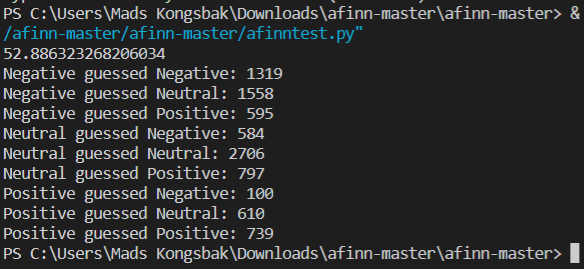
\includegraphics[width=0.9\textwidth]{Images/AfinnResult}
	\caption{Results running Afinn without emoticons}
\end{figure}

\begin{figure}[H]
	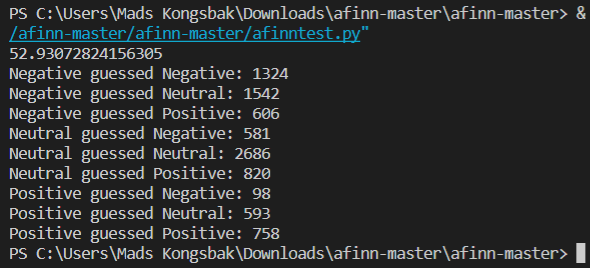
\includegraphics[width=0.9\textwidth]{Images/AfinnResultEmoticons}
	\caption{Results running Afinn with emoticons}
\end{figure}

\subsection{Baseline Classifier F1 Score Calculation}

\begin{table}[H]
	\begin{tabular}{@{}lllll@{}}
		\toprule
		& & \multicolumn{2}{c}{Predicted} \\\cmidrule{2-4}
		Actual & & Negative & Other & \\ \midrule
		Negative & & 0 True Positives & 3472 False Negatives & \\
		Other  & & 0 False Positives & 5536 True Negatives & \\ \bottomrule
	\end{tabular}
	\centering
	\caption{Table of Confusion for Negatives}
	\label{blneg}
\end{table}

\[F1 = \dfrac{2\cdot0}{(2\cdot0) + 3472 + 0} = 0\]


\begin{table}[H]
	\begin{tabular}{@{}lllll@{}}
		\toprule
		& & \multicolumn{2}{c}{Predicted} \\\cmidrule{2-4}
		Actual & & Neutral & Other & \\ \midrule
		Neutral & & 4087 True Positives & 0 False Negatives & \\
		Other  & & 4927 False Positives & 0 True Negatives & \\ \bottomrule
	\end{tabular}
	\centering
	\caption{Table of Confusion for Neutrals}
	\label{blneu}
\end{table}

\[F1 = \dfrac{2\cdot4087}{(2\cdot4087) + 4927 + 0} = 0.62420771286\]


\begin{table}[H]
	\begin{tabular}{@{}lllll@{}}
		\toprule
		& & \multicolumn{2}{c}{Predicted} \\\cmidrule{2-4}
		Actual & & Positive & Other & \\ \midrule
		Positive & & 0 True Positives & 1449 False Negatives & \\
		Other  & & 0 False Positives & 7559 True Negatives & \\ \bottomrule
	\end{tabular}
	\centering
	\caption{Table of Confusion for Positives}
	\label{blpos}
\end{table}


\[F1 = \dfrac{2\cdot0}{(2\cdot0) + 1449 + 0} = 0\]

\[F1 Average = \dfrac{0.62420771286+0+0}{3} = 0.20806923762\]

\subsection{Random Classifier F1 Score Calculation}

\begin{table}[H]
	\begin{tabular}{@{}lllll@{}}
		\toprule
		& & \multicolumn{2}{c}{Predicted} \\\cmidrule{2-4}
		Actual & & Negative & Other & \\ \midrule
		Negative & & 1167 True Positives & 2305 False Negatives & \\
		Other  & & 1905 False Positives & 3631 True Negatives & \\ \bottomrule
	\end{tabular}
	\centering
	\caption{Table of Confusion for Negatives}
	\label{randomneg}
\end{table}

\[F1 = \dfrac{2\cdot1167}{(2\cdot1167) + 2305 + 1905} = 0.35666259168\]


\begin{table}[H]
	\begin{tabular}{@{}lllll@{}}
		\toprule
		& & \multicolumn{2}{c}{Predicted} \\\cmidrule{2-4}
		Actual & & Neutral & Other & \\ \midrule
		Neutral & & 1361 True Positives & 2726 False Negatives & \\
		Other  & & 1630 False Positives & 3291 True Negatives & \\ \bottomrule
	\end{tabular}
	\centering
	\caption{Table of Confusion for Neutrals}
	\label{randomneu}
\end{table}

\[F1 = \dfrac{2\cdot1361}{(2\cdot1361) + 1630 + 2726} = 0.38457191297\]


\begin{table}[H]
	\begin{tabular}{@{}lllll@{}}
		\toprule
		& & \multicolumn{2}{c}{Predicted} \\\cmidrule{2-4}
		Actual & & Positive & Other & \\ \midrule
		Positive & & 453 True Positives & 2492 False Negatives & \\
		Other  & & 996 False Positives & 5067 True Negatives & \\ \bottomrule
	\end{tabular}
	\centering
	\caption{Table of Confusion for Positives}
	\label{randompos}
\end{table}


\[F1 = \dfrac{2\cdot453}{(2\cdot453) + 996 + 2492} = 0.20619025944\]

\[F1 Average = \dfrac{0.35666259168+0.38457191297+0.20619025944}{3} = 0.31580825469\]

\subsection{Afinn Classifier F1 Score Calculation}

\begin{table}[H]
	\begin{tabular}{@{}lllll@{}}
		\toprule
		& & \multicolumn{2}{c}{Predicted} \\\cmidrule{2-4}
		Actual & & Negative & Other & \\ \midrule
		Negative & & 1319 True Positives & 2153 False Negatives & \\
		Other  & & 684 False Positives & 4852 True Negatives & \\ \bottomrule
	\end{tabular}
	\centering
	\caption{Table of Confusion for Negatives}
	\label{afinnneg}
\end{table}

\[F1 = \dfrac{2\cdot1319}{(2\cdot1319) + 684 + 2153} = 0.48182648401\]


\begin{table}[H]
	\begin{tabular}{@{}lllll@{}}
		\toprule
		& & \multicolumn{2}{c}{Predicted} \\\cmidrule{2-4}
		Actual & & Neutral & Other & \\ \midrule
		Neutral & & 2706 True Positives & 1381 False Negatives & \\
		Other  & & 2168 False Positives & 2753 True Negatives & \\ \bottomrule
	\end{tabular}
	\centering
	\caption{Table of Confusion for Neutrals}
	\label{rbneu}
\end{table}

\[F1 = \dfrac{2\cdot2706}{(2\cdot2706) + 2168 + 1381} = 0.60395045195\]


\begin{table}[H]
	\begin{tabular}{@{}lllll@{}}
		\toprule
		& & \multicolumn{2}{c}{Predicted} \\\cmidrule{2-4}
		Actual & & Positive & Other & \\ \midrule
		Positive & & 739 True Positives & 710 False Negatives & \\
		Other  & & 1392 False Positives & 6167 True Negatives & \\ \bottomrule
	\end{tabular}
	\centering
	\caption{Table of Confusion for Positives}
	\label{rbpos}
\end{table}


\[F1 = \dfrac{2\cdot739}{(2\cdot739) + 710 + 1392} = 0.41284916201\]

\[F1 Average = \dfrac{0.48182648401+0.60395045195+0.41284916201}{3} = 0.49954203265\]

\subsection{Lexical Analysis F1 Score Calculation}

\begin{table}[H]
	\begin{tabular}{@{}lllll@{}}
		\toprule
		& & \multicolumn{2}{c}{Predicted} \\\cmidrule{2-4}
		Actual & & Negative & Other & \\ \midrule
		Negative & & 1720 True Positives & 1752 False Negatives & \\
		Other  & & 808 False Positives & 4728 True Negatives & \\ \bottomrule
	\end{tabular}
	\centering
	\caption{Table of Confusion for Negatives}
	\label{rbneg}
\end{table}

\[F1 = \dfrac{2\cdot1720}{(2\cdot1720) + 808 + 1752} = 0.57333333333\]


\begin{table}[H]
	\begin{tabular}{@{}lllll@{}}
		\toprule
		& & \multicolumn{2}{c}{Predicted} \\\cmidrule{2-4}
		Actual & & Neutral & Other & \\ \midrule
		Neutral & & 2600 True Positives & 1487 False Negatives & \\
		Other  & & 1823 False Positives & 3098 True Negatives & \\ \bottomrule
	\end{tabular}
	\centering
	\caption{Table of Confusion for Neutrals}
	\label{rbneu}
\end{table}

\[F1 = \dfrac{2\cdot2600}{(2\cdot2600) + 1823 + 1487} = 0.61104582843\]


\begin{table}[H]
	\begin{tabular}{@{}lllll@{}}
		\toprule
		& & \multicolumn{2}{c}{Predicted} \\\cmidrule{2-4}
		Actual & & Positive & Other & \\ \midrule
		Positive & & 749 True Positives & 700 False Negatives & \\
		Other  & & 1308 False Positives & 6251 True Negatives & \\ \bottomrule
	\end{tabular}
	\centering
	\caption{Table of Confusion for Positives}
	\label{rbpos}
\end{table}


\[F1 = \dfrac{2\cdot749}{(2\cdot749) + 700 + 1308} = 0.42726754135\]

\[F1 Average = \dfrac{0.61104582843 + 0.57333333333 + 0.42726754135}{3} = 0.5372155677\]